% !TEX program = pdflatex
\documentclass[11pt]{article}
\setlength{\textwidth}{6.5in}
\setlength{\oddsidemargin}{0pt}
\setlength{\evensidemargin}{0pt}
\setlength{\textheight}{9in}
\setlength{\topmargin}{0pt}
\addtolength{\topmargin}{-\headheight}
\addtolength{\topmargin}{-\headsep}
\ifdefined\pdfpagewidth \pdfpagewidth=8.5in \pdfpageheight=11in \fi
\ifdefined\pagewidth \pagewidth=8.5in \pageheight=11in \fi
\usepackage{amsmath,amssymb}
\usepackage{array}
\usepackage{booktabs}
\usepackage[tableposition=top]{caption}
\usepackage{longtable}
\usepackage{enumitem}
\usepackage{tikz}
\usepackage{pgfplots}
\pgfplotsset{compat=1.18}
\emergencystretch=3em

% ---- notation ---------------------------------------------------------------
\newcommand{\um}{\,$\mu$m}
\newcommand{\kms}{km\,s$^{-1}$}
\newcommand{\mJyb}{mJy\,beam$^{-1}$}
\newcommand{\lnu}{erg\,s$^{-1}$\,Hz$^{-1}$}
\newcommand{\sci}[2]{#1\times10^{#2}}
\newcommand{\Msun}{M_\odot}
\newcommand{\Rsun}{R_\odot}

% ---- front matter -----------------------------------------------------------
\title{A Variable, Circularly Polarised 144\,MHz Source\\ on the A2V Star 50 Cassiopeiae}
\author{Charles C. Norton}
\date{}

\begin{document}
\maketitle

\begin{abstract}
An A star has no convective envelope to drive a corona, and the A stars LOFAR has
detected at $144$\,MHz, two magnetic chemically peculiar stars, show circular
polarisation well below $60$ per cent. In the per-pointing Stokes~V images of the third
data release of the LOFAR Two-metre Sky Survey, 50~Cas (HD~12216, A2V, $48$\,pc,
$V=3.95$) is the one A star within $50$\,pc of $129$ measured that carries a polarised
source. Three epochs cover it. On 2020 September 28 and 2022 April 10 a source of $1.7$
and $2.6$\,\mJyb\ stands on the star with Stokes~V about $60$ per cent of its peak, and
the two epochs give $+1.13\pm0.14$\,\mJyb\ at the star's position ($7.9\sigma$); on
2022 January 6 the star's position holds $+0.08\pm0.15$\,\mJyb, so the polarised flux
changes between epochs ($\chi^2=30$ for $2$ degrees of freedom). At $48$\,pc the April
source has a spectral luminosity of $\sci{7}{15}$\,\lnu, and confined to the star's own
radius it would have a brightness temperature of $\sci{7}{11}$\,K. TESS's light curves of
nine sectors from 2019 to 2024 hold a stable double wave with unequal maxima at
$1.596538$\,d, semi-amplitudes of $2.88$\,mmag at half the period and $1.54$\,mmag at
the period, which Hipparcos recorded at its first harmonic; at the star's radius of
$2.98\,\Rsun$ the period gives an equatorial speed of $94$\,\kms, against a measured
$v\sin i$ of $85$--$91$\,\kms. Coud\'e spectra of 1992 hold a companion on that period
below about $0.17\,\Msun$, which cannot make the light curve's term at the period. The
star reads as a magnetic A star with surface spots turning in $1.6$ days, whose
electron-cyclotron emission is beamed across Earth at some rotational phases; no
measurement of its field exists, and one would settle it.
\end{abstract}

% =============================================================================
\section{Introduction}\label{sec:intro}
% =============================================================================

Main-sequence A stars lack the convective envelopes that power the coronae of cooler
stars, and their radio emission comes from the magnetic chemically peculiar stars,
whose large-scale dipolar fields trap electrons in a magnetosphere. These emit
gyrosynchrotron radiation at gigahertz frequencies, with luminosities that scale with
the field and the rotation~\cite{Leto2021}, and some emit coherent pulses by the
electron-cyclotron maser, strongly circularly polarised and beamed, which arrive at the
rotational phases where the line of sight crosses the magnetic equator, as first seen in
CU~Vir~\cite{Trigilio2000}. At $144$\,MHz, LOFAR detected two magnetic chemically
peculiar stars, BP~Boo and $\alpha^2$~CVn, in total intensity, with circular
polarisation below $60$ per cent~\cite{Hajduk2022}. The strongly circularly polarised
stellar sources at these frequencies are active M dwarfs~\cite{Callingham2021} and
RS~CVn binaries~\cite{Toet2021}, catalogued over a quarter of the northern sky by the
circularly polarised survey of LOFAR's second data release~\cite{Callingham2023}.

The third data release of the LOFAR Two-metre Sky Survey (LoTSS-DR3) covers $88$ per
cent of the northern sky and publishes a Stokes~V image of each pointing's
epoch~\cite{Shimwell2026}. Read at the nearest stars, those images show the flare stars
and active binaries already known, and one A star. This note reports that star, 50~Cas,
and what the archives give for its nature.

\subsection{Contributions}
\begin{enumerate}[leftmargin=*,itemsep=1pt]
\item A circularly polarised, variable $144$\,MHz source on 50~Cas in three epochs of
LoTSS-DR3, the only one among $129$ A and early-F stars within $50$\,pc.
\item The star's $1.5965$\,d cycle in nine TESS sectors and its consistency with the
measured rotational broadening, and the limit that spectra of 1992 set on a companion
on that cycle.
\end{enumerate}

% =============================================================================
\section{50 Cassiopeiae}\label{sec:star}
% =============================================================================

50~Cas (HD~12216, HR~580, HIP~9598) is a naked-eye A2V star. Gaia DR3~\cite{Gaia2023}
gives a parallax of $20.84\pm0.19$\,mas ($48.0$\,pc), $G=3.95$,
$G_\mathrm{BP}-G_\mathrm{RP}=0.06$, a renormalised unit weight error of $3.2$, which is
common at $G\approx4$, no non-single-star solution and no radial velocity, and from its
spectrophotometry an effective temperature of $9060$\,K, a radius of $2.98\,\Rsun$, a
luminosity of $54\,L_\odot$, a mass of $2.4\,\Msun$ and an age of $0.5$\,Gyr; the
debris-disc survey of Rieke et al.\ gives it $320$\,Myr~\cite{Rieke2005}. Its projected
rotational velocity is $85$\,\kms~\cite{AbtMorrell1995} and $90$--$91$\,\kms~\cite{Royer2002,Royer2007}.
Three classifications of 1954--1960 collected by SIMBAD read A1\,V\,SB. The catalogue of
Ap, HgMn and Am stars~\cite{RensonManfroid2009} does not list it. It was among the targets
of a magnetic survey of the bright northern main-sequence stars~\cite{Monin2002}, and the
compilation of averaged effective fields of Bychkov et al.~\cite{Bychkov2003}, which
carries that survey's measurements of $28$ stars, holds none of 50~Cas. The
Hipparcos--Gaia proper-motion anomaly stands at a signal-to-noise ratio of
$1.5$--$1.7$~\cite{Kervella2022}. Koen and Eyer found a period in its Hipparcos
photometry, $1.25273$\,d$^{-1}$ at $3$\,mmag~\cite{KoenEyer2002}. IRAS's $25$\um\ flux
reads $1.26$ times the photosphere~\cite{Rieke2005}, listed among the less certain excess
stars~\cite{CottenSong2016}, while AllWISE's W3 and W4, $3.91$ and $3.86$\,mag against
2MASS $K_s=3.92$, allow no excess above about five per cent at $12$ and $22$\um. No other
Gaia source lies within $24''$; the nearest, at $33''$ and $51''$, are $10.5$\,mag
fainter. The star is a target of Breakthrough Listen's nearby-star
survey~\cite{Isaacson2017}.

% =============================================================================
\section{Data and method}\label{sec:method}
% =============================================================================

\paragraph{LoTSS-DR3.} Each DR3 pointing is an $8$\,h observation of one epoch. The
ASTRON VO's table of DR3 pointings gives the midpoint of each observation, and the SURF
Data Repository holds each pointing's products as tar archives, from which the $6''$
dirty Stokes~I and V images and the $6''$ restored Stokes~I image with astrometric
corrections were read by HTTP byte range, a patch around the star alone, and put on
DR3's flux scale by the factor the release gives for the pointing. The search that found
50~Cas measured Stokes~V at the $246$ Hipparcos stars within $50$\,pc with
$-0.05<B-V<0.32$ north of $-1^\circ$ in their two nearest pointings, each star carried to
the pointing's epoch, its noise from the robust scatter of the annulus $12''$--$30''$
out, positions $22.5''$ away serving as the null; $61$ of the $190$ measured carry a
placeholder colour or an absolute magnitude fainter than $3.5$ and are later stars,
leaving $129$ A and early-F stars at a median $5\sigma$ limit of $0.54$\,mJy. For 50~Cas
every pointing within $3^\circ$ was read, three of which cover it.

\paragraph{TESS.} The two-minute PDCSAP light curves of sectors 18, 19, 25, 52, 58, 59,
78, 79 and 86, $141552$ cadences of quality zero from 2019 to 2024, in mmag about each
sector's median, were fitted with a fundamental frequency and its first three harmonics
and one offset per sector over a fine grid of frequencies, the frequency's error from
the curvature of $\chi^2$ with the residual scatter as the noise. The ephemeris for
phases is $0.62635569$\,d$^{-1}$ with phase zero at BJD~2457000.

\paragraph{DAO spectra.} The Canadian Astronomy Data Centre holds $19$ McKellar coud\'e
spectra of 50~Cas from the Dominion Astrophysical Observatory's $1.2$\,m telescope, from
1990, 1992, 2000 and 2006. The $13$ of 1992 December 18 cover $3.12$\,h on one setup at
$2.4$\,\AA\,mm$^{-1}$ near $4486$--$4558$\,\AA, with $39$ flats and Th--Ar arcs
interleaved. Each exposure was divided by the median flat and cross-correlated with the
series mean, and the arcs' drift of $0.8$\,\kms\ through the night was removed.

% =============================================================================
\section{Results}\label{sec:results}
% =============================================================================

\subsection{The 144 MHz source}

50~Cas is the only one of the $129$ A and early-F stars above $3\sigma$ in Stokes~V, at
$+5.4\sigma$ over its two nearest pointings. Table~\ref{tab:lofar} gives the three
epochs. On 2022 April 10 the dirty images hold a Stokes~I peak of $2.58\pm0.28$\,\mJyb\
$1.5''$ from the star and Stokes~V of $+1.53\pm0.19$\,\mJyb\ there, a fraction of $0.59$;
the restored image with astrometric corrections places the Stokes~I peak $0.07''$ from
the star at a signal-to-noise ratio of $16.5$. On 2020 September 28 the source stands at
$1.73\pm0.29$\,\mJyb\ with Stokes~V of $+1.16\pm0.22$\,\mJyb\ at the peak, a fraction of
$0.67$. On 2022 January 6, between them, nothing stands at the star: Stokes~I reaches
$1.8\sigma$ and Stokes~V at the star's position is $+0.08\pm0.15$\,\mJyb. Read at the
star's position, the two epochs with the source give $+1.13\pm0.14$\,\mJyb\
($7.9\sigma$), and the three epochs are inconsistent with one value, $\chi^2=30.3$ for
$2$ degrees of freedom.

\begin{table}[t]
\centering\small
\caption{50~Cas in the per-pointing images of LoTSS-DR3: the pointing, the date of the
observation's midpoint, the star's distance from the pointing centre, DR3's flux-scale
factor, the phase range of the $8$\,h observation on the TESS ephemeris, the dirty
Stokes~I peak within $4.5''$ of the star and its offset, and Stokes~V at that peak and at
the star's position, all on DR3's flux scale.}
\label{tab:lofar}
\setlength{\tabcolsep}{4.5pt}
\begin{tabular}{llrrcrrrr}
\toprule
Pointing & Date & Offset ($^\circ$) & Scale & Phase & $I$ (\mJyb) & ($''$) & $V_\mathrm{peak}$ & $V_\mathrm{star}$ \\
\midrule
P037+71 & 2020 Sep 28 & $2.27$ & $1.307$ & $0.64$--$0.85$ & $1.73\pm0.29$ & $3.4$ & $+1.16$ & $+0.77\pm0.22$ \\
P032+74 & 2022 Jan 6 & $1.49$ & $0.958$ & $0.75$--$0.96$ & $0.30\pm0.17$ & $2.1$ & $0.00$ & $+0.08\pm0.15$ \\
P029+71 & 2022 Apr 10 & $1.20$ & $1.084$ & $0.40$--$0.61$ & $2.58\pm0.28$ & $1.5$ & $+1.53$ & $+1.38\pm0.19$ \\
\bottomrule
\end{tabular}
\end{table}

At $48.0$\,pc the April flux density corresponds to a spectral luminosity of
$\sci{7.1}{15}$\,\lnu, $\sci{3.8}{15}$\,\lnu\ of it circularly polarised. Emission
confined to a region of the star's radius would have a brightness temperature of
$\sci{7}{11}$\,K, and one of five stellar radii $\sci{3}{10}$\,K. Nothing lies within
$60''$ in the ROSAT All-Sky Survey catalogues, nor in NVSS or TGSS at the star, and the
four VLASS quick-look epochs of 2017--2026 hold nothing above $1.8\sigma$ at $3$\,GHz,
$5\sigma$ limits of $0.8$--$1.1$\,mJy or $\sci{2}{15}$ to $\sci{3}{15}$\,\lnu.

\subsection{The 1.6-day cycle}

The TESS fit gives $f=0.62635527\pm0.00000006$\,d$^{-1}$, a period of $1.596538$\,d,
with semi-amplitudes of $1.54$\,mmag at $f$, $2.88$\,mmag at $2f$ and $0.11$ and
$0.07$\,mmag at $3f$ and $4f$, and residuals of $0.40$\,mmag per two-minute cadence. Each
sector alone gives $1.45$--$1.59$\,mmag at $f$ and $2.81$--$2.96$\,mmag at $2f$, so the
curve has held its shape for five years. Folded (Figure~\ref{fig:fold}), it is a double
wave with unequal maxima, $4.3$\,mmag above the mean at phase $0.27$ and $1.4$\,mmag at
$0.80$, and unequal minima, $3.7$\,mmag below at $0.53$ and $2.1$\,mmag at $0.02$. The
frequency Hipparcos found is $2f$. No Gaia source within $90''$ is brighter than
$G=14.5$, and none can carry a modulation of $0.7$ per cent of a fourth-magnitude
star's light, so the cycle is 50~Cas's own.

\begin{figure}[t]
\centering
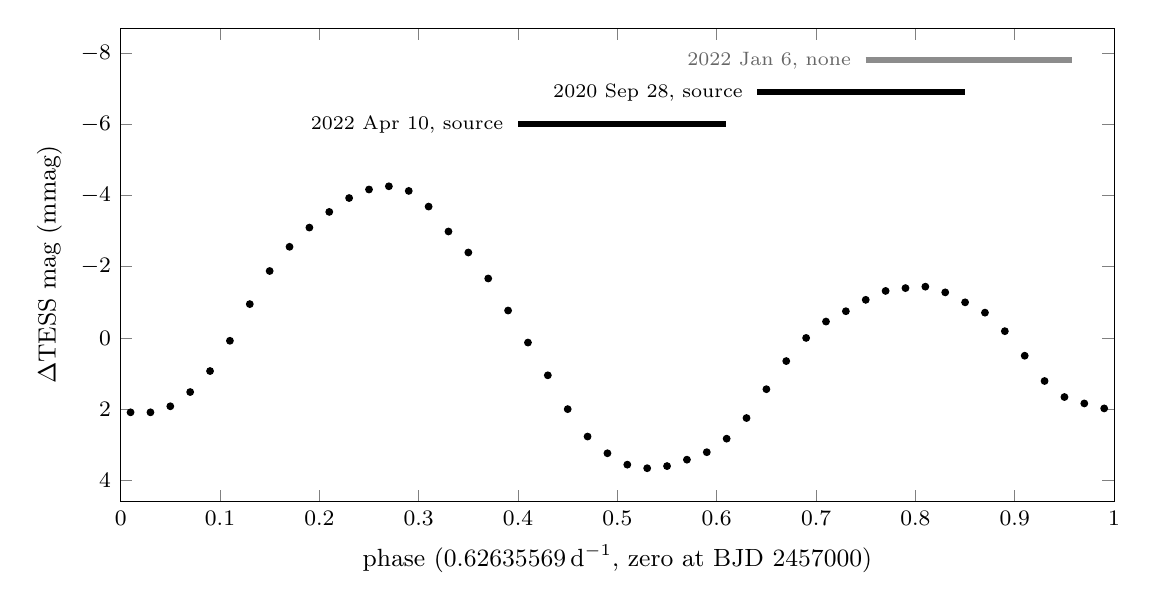
\begin{tikzpicture}
\begin{axis}[width=0.86\textwidth,height=0.46\textwidth,xmin=0,xmax=1,ymin=-8.7,ymax=4.6,y dir=reverse,
  xlabel={phase ($0.62635569$\,d$^{-1}$, zero at BJD 2457000)},ylabel={$\Delta$TESS mag (mmag)},
  tick label style={font=\footnotesize},label style={font=\small}]
\addplot[only marks,mark=*,mark size=1.2pt,black] coordinates {(0.01,2.09) (0.03,2.09) (0.05,1.92) (0.07,1.52) (0.09,0.93) (0.11,0.08) (0.13,-0.95) (0.15,-1.88) (0.17,-2.56) (0.19,-3.10) (0.21,-3.54) (0.23,-3.93) (0.25,-4.17) (0.27,-4.26) (0.29,-4.13) (0.31,-3.69) (0.33,-2.99) (0.35,-2.40) (0.37,-1.67) (0.39,-0.77) (0.41,0.13) (0.43,1.05) (0.45,2.00) (0.47,2.77) (0.49,3.24) (0.51,3.56) (0.53,3.66) (0.55,3.60) (0.57,3.42) (0.59,3.21) (0.61,2.83) (0.63,2.25) (0.65,1.44) (0.67,0.65) (0.69,-0.00) (0.71,-0.46) (0.73,-0.75) (0.75,-1.07) (0.77,-1.32) (0.79,-1.40) (0.81,-1.44) (0.83,-1.28) (0.85,-1.00) (0.87,-0.71) (0.89,-0.19) (0.91,0.50) (0.93,1.21) (0.95,1.66) (0.97,1.84) (0.99,1.98)};
\draw[black,line width=2.2pt] (axis cs:0.400,-6.0) -- (axis cs:0.609,-6.0);
\node[font=\scriptsize,anchor=east] at (axis cs:0.395,-6.0) {2022 Apr 10, source};
\draw[black,line width=2.2pt] (axis cs:0.641,-6.9) -- (axis cs:0.850,-6.9);
\node[font=\scriptsize,anchor=east] at (axis cs:0.636,-6.9) {2020 Sep 28, source};
\draw[black!45,line width=2.2pt] (axis cs:0.750,-7.8) -- (axis cs:0.958,-7.8);
\node[font=\scriptsize,anchor=east,text=black!60] at (axis cs:0.745,-7.8) {2022 Jan 6, none};
\end{axis}
\end{tikzpicture}
\caption{The TESS light curve of 50~Cas over nine sectors of 2019--2024, folded on the
ephemeris and binned in $50$ phase bins (errors smaller than the points), brighter
upward; the bars mark the phases each $8$\,h LoTSS-DR3 observation covered, black where
the polarised source was present and grey where it was not.}
\label{fig:fold}
\end{figure}

At the star's radius of $2.98\,\Rsun$, turning once in $1.5965$\,d moves the equator at
$94$\,\kms, and the measured $v\sin i$ of $85$--$91$\,\kms\ then puts the inclination
above about $65^\circ$, the star seen nearly equator-on. Turning once in half the period
would need $188$\,\kms\ at the equator and an inclination near $30^\circ$, and would
leave no light at $f$ itself.

\subsection{A companion on the cycle}

The 1992 series runs from phase $0.297$ to $0.379$, and across its $3.12$\,h the
spectrum moves by $+1.0\pm0.4$\,\kms\ (a slope of $+0.31\pm0.12$\,\kms\,h$^{-1}$ with a
scatter of $0.38$\,\kms). If the cycle were an orbit with conjunctions at the light
minima, a companion would change the A star's velocity by $0.15$ to $0.21$ times its
semi-amplitude $K$ across those phases, so $K$ lies below about $15$\,\kms\ ($2\sigma$)
and the companion below about $0.17\,\Msun$ at an inclination near $90^\circ$. Such a
companion can make the $2.88$\,mmag ellipsoidal term at $2f$, but not the $1.54$\,mmag
term at $f$: an M dwarf $8\,\Rsun$ from a $54\,L_\odot$ star reflects about $0.15$\,mmag
and Doppler beaming at $15$\,\kms\ gives about $0.2$\,mmag. A companion of A type would
shift the lines by tens of \kms\ across the series and double them, and does neither. The
two spectra of 2000 September, at phases $0.86$ and $0.57$, differ by
$5.5\pm2$\,\kms\ with the sign along the pixel axis undetermined, an orbit's $K$ of about
$7$\,\kms\ or the line-profile change that surface spots make.

% =============================================================================
\section{Discussion}\label{sec:discussion}
% =============================================================================

The polarised fraction, about $60$ per cent, and the brightness temperature, $10^{10}$
to $10^{12}$\,K for regions of one to five stellar radii, point to coherent emission, and
the electron-cyclotron maser is the coherent process that a magnetised star sustains.
Emission at the fundamental of the gyrofrequency at $144$\,MHz needs about $51$\,G where
it forms, which a dipole of a kilogauss at the pole holds at about $2.7$ stellar radii.

Two readings fit what the archives give. In the first, 50~Cas is a magnetic A star: the
light curve, a double wave with unequal maxima that has kept its shape for five years, is
that of abundance spots fixed on the surface of a magnetic chemically peculiar star
turning nearly equator-on, and the radio emission is its magnetosphere's
electron-cyclotron maser, beamed so that Earth sees it at some phases and not others, as
CU~Vir's pulses are~\cite{Trigilio2000}. The three epochs fit a pulse near phase $0.62$
lasting about a tenth of a cycle, at the end of the April observation and the start of
the September one and outside the January one, and they fit as well an emission that
changes from year to year. The two LOFAR detections of magnetic chemically peculiar
stars at $144$\,MHz are in total intensity, with circular polarisation below $60$ per
cent~\cite{Hajduk2022}, so this would be the first of their class seen there by its
coherent emission.

In the second reading the radio source is an unseen companion below $0.17\,\Msun$: a
late M dwarf held in a $1.6$\,d orbit would rotate fast enough to be active, and LOFAR
hears active M dwarfs and RS~CVn binaries by their coherent, strongly polarised
emission~\cite{Callingham2021,Toet2021}. The $1.54$\,mmag term at $f$ still needs an
inhomogeneous surface on the A star, which neither reflection nor beaming supplies, so
the light curve speaks for the A star's own spots under either reading. A measurement of
the longitudinal field by spectropolarimetry would decide between them, a field of
hundreds of gauss marking the star as magnetic; a high-resolution spectrum would show
whether its abundances are peculiar, and time-resolved $144$\,MHz data, which the DR3
visibilities hold, would show whether the emission comes in pulses at fixed phases.

% =============================================================================
\section{Related work}\label{sec:related}
% =============================================================================

Radio emission from magnetic chemically peculiar stars has been studied at gigahertz
frequencies for decades, with a scaling of the incoherent luminosity with field and
rotation~\cite{Leto2021} and coherent pulses since CU~Vir~\cite{Trigilio2000}; at
$144$\,MHz the LoTSS second data release yielded two detections in total
intensity~\cite{Hajduk2022}, and its circularly polarised catalogue covered areas that do
not include 50~Cas~\cite{Callingham2023}. The photometric period of 50~Cas was found in
the Hipparcos photometry~\cite{KoenEyer2002}, and its rotational broadening is measured
in the surveys of A-star rotation~\cite{AbtMorrell1995,Royer2002,Royer2007}. No earlier
radio detection of 50~Cas, and no measurement of its magnetic field, is found in the
literature.

% =============================================================================
\section{Conclusion}\label{sec:conclusion}
% =============================================================================

50~Cas, an A2V star at $48$\,pc, carries a $144$\,MHz source with circular
polarisation of about $60$ per cent in two of the three LoTSS-DR3 epochs that cover it,
absent in the third, at a luminosity of $\sci{7}{15}$\,\lnu\ and a brightness temperature
that requires coherent emission. The star turns in $1.5965$\,d nearly equator-on, its
light a stable double wave with unequal maxima, and any companion on that cycle is below
about $0.17\,\Msun$. It reads as a magnetic A star whose electron-cyclotron emission is
beamed across Earth at some rotational phases, with an active low-mass companion as the
alternative. A spectropolarimetric measurement of its field would settle which.

\section*{Acknowledgements}

This work uses LoTSS-DR3 data from the LOFAR telescope, designed and constructed by
ASTRON, with its products served by the ASTRON VO and the SURF Data Repository; data
from the TESS mission, funded by NASA's Science Mission Directorate, obtained from the
Mikulski Archive for Space Telescopes; data from the European Space Agency mission
Gaia, processed by the Gaia Data Processing and Analysis Consortium, funded by national
institutions, in particular those participating in the Gaia Multilateral Agreement;
spectra of the Dominion Astrophysical Observatory, National Research Council Canada,
served by the Canadian Astronomy Data Centre; the VLA Sky Survey of the National Radio
Astronomy Observatory; the ROSAT All-Sky Survey, IRAS, 2MASS and WISE catalogues; and the
SIMBAD and VizieR services at CDS, Strasbourg.

\begin{thebibliography}{99}\small\raggedright
\setlength{\itemsep}{1pt}

\bibitem{Leto2021}
P.~Leto, C.~Trigilio, J.~Krti\v{c}ka, et al., A scaling relationship for non-thermal radio
emission from ordered magnetospheres: from the top of the main sequence to planets,
\emph{Mon. Not. R. Astron. Soc.} \textbf{507}, 1979 (2021).

\bibitem{Trigilio2000}
C.~Trigilio, P.~Leto, F.~Leone, et al., Coherent radio emission from the magnetic
chemically peculiar star CU Virginis, \emph{Astron. Astrophys.} \textbf{362}, 281 (2000).

\bibitem{Hajduk2022}
M.~Hajduk, P.~Leto, H.~Vedantham, et al., Radio detection of chemically peculiar stars
with LOFAR, \emph{Astron. Astrophys.} \textbf{665}, A152 (2022).

\bibitem{Callingham2021}
J.~R. Callingham, H.~K. Vedantham, T.~W. Shimwell, et al., The population of M dwarfs
observed at low radio frequencies, \emph{Nat. Astron.} \textbf{5}, 1233 (2021).

\bibitem{Toet2021}
S.~E.~B. Toet, H.~K. Vedantham, J.~R. Callingham, et al., Coherent radio emission from a
population of RS Canum Venaticorum systems, \emph{Astron. Astrophys.} \textbf{654}, A21
(2021).

\bibitem{Callingham2023}
J.~R. Callingham, T.~W. Shimwell, H.~K. Vedantham, et al., V-LoTSS: the circularly
polarised LOFAR Two-metre Sky Survey, \emph{Astron. Astrophys.} \textbf{670}, A124
(2023).

\bibitem{Shimwell2026}
T.~W. Shimwell, M.~J. Hardcastle, C.~Tasse, et al., The LOFAR Two-metre Sky Survey: VII.
Third data release, \emph{Astron. Astrophys.} \textbf{707}, A198 (2026).

\bibitem{Gaia2023}
Gaia Collaboration, A.~Vallenari, A.~G.~A. Brown, et al., Gaia Data Release 3: summary
of the content and survey properties, \emph{Astron. Astrophys.} \textbf{674}, A1 (2023).

\bibitem{Rieke2005}
G.~H. Rieke, K.~Y.~L. Su, J.~A. Stansberry, et al., Decay of planetary debris disks,
\emph{Astrophys. J.} \textbf{620}, 1010 (2005).

\bibitem{AbtMorrell1995}
H.~A. Abt and N.~I. Morrell, The relation between rotational velocities and spectral
peculiarities among A-type stars, \emph{Astrophys. J. Suppl.} \textbf{99}, 135 (1995).

\bibitem{Royer2002}
F.~Royer, S.~Grenier, M.-O. Baylac, A.~E. G\'omez and J.~Zorec, Rotational velocities
of A-type stars. II. Measurement of $v\sin i$ in the northern hemisphere,
\emph{Astron. Astrophys.} \textbf{393}, 897 (2002).

\bibitem{Royer2007}
F.~Royer, J.~Zorec and A.~E. G\'omez, Rotational velocities of A-type stars. III.
Velocity distributions, \emph{Astron. Astrophys.} \textbf{463}, 671 (2007).

\bibitem{RensonManfroid2009}
P.~Renson and J.~Manfroid, Catalogue of Ap, HgMn and Am stars, \emph{Astron. Astrophys.}
\textbf{498}, 961 (2009).

\bibitem{Monin2002}
D.~N. Monin, S.~N. Fabrika and G.~G. Valyavin, Magnetic survey of bright northern main
sequence stars, \emph{Astron. Astrophys.} \textbf{396}, 131 (2002).

\bibitem{Bychkov2003}
V.~D. Bychkov, L.~V. Bychkova and J.~Madej, Catalogue of averaged stellar effective
magnetic fields. I. Chemically peculiar A and B type stars, \emph{Astron. Astrophys.}
\textbf{407}, 631 (2003).

\bibitem{Kervella2022}
P.~Kervella, F.~Arenou and F.~Th\'evenin, Stellar and substellar companions from Gaia
EDR3: proper-motion anomaly and resolved common proper-motion pairs, \emph{Astron.
Astrophys.} \textbf{657}, A7 (2022).

\bibitem{KoenEyer2002}
C.~Koen and L.~Eyer, New periodic variables from the Hipparcos epoch photometry,
\emph{Mon. Not. R. Astron. Soc.} \textbf{331}, 45 (2002).

\bibitem{CottenSong2016}
T.~H. Cotten and I.~Song, A comprehensive census of nearby infrared excess stars,
\emph{Astrophys. J. Suppl.} \textbf{225}, 15 (2016).

\bibitem{Isaacson2017}
H.~Isaacson, A.~P.~V. Siemion, G.~W. Marcy, et al., The Breakthrough Listen search for
intelligent life: target selection of nearby stars and galaxies, \emph{Publ. Astron.
Soc. Pac.} \textbf{129}, 054501 (2017).

\end{thebibliography}

\end{document}
